\section{Herleitungen mittels konkreten Beispielen}
\subsection{Brechungsgesetz von Snellius \label{brechungsgesetz}}
Aus dem Fermatschen Prinzip l"asst sich das Brechungsgesetz von Snellius
herleiten.
Das Licht legt den Weg vom Startpunkt $P_0$ "uber den Brechungspunkt $P_1$ 
nach dem Endpunkt $P_2$ zur"uck \cite{Wikipedia}, siehe \figref{Ab:brechung} .
\begin{figure}[h]
\begin{center}
	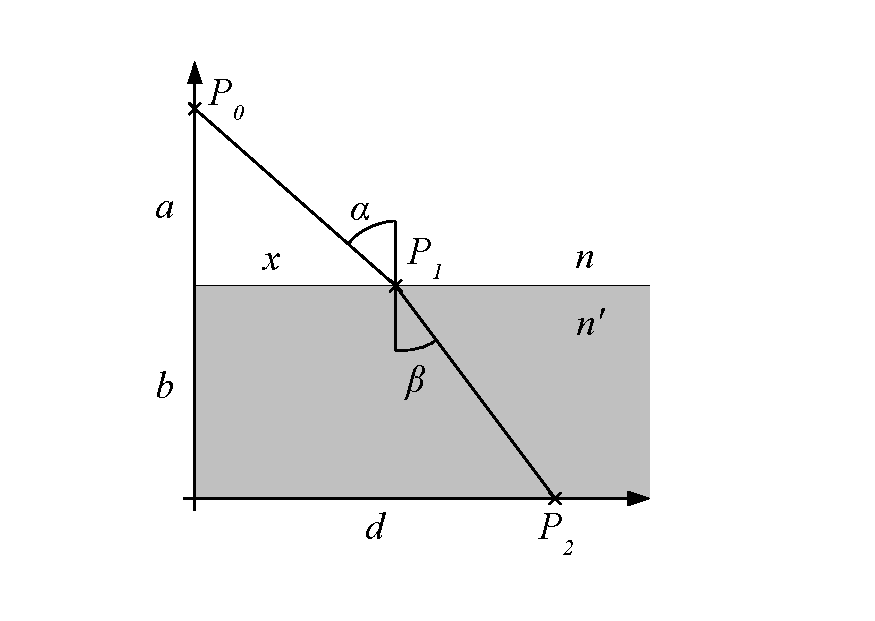
\includegraphics[width=0.7\textwidth]{licht/picture/Brechung.pdf}
	\caption{Skizze des Brechungsgesetzes von Snellius}
	\label{Ab:brechung}
\end{center}
\end{figure}
Dadurch kann die zur"uckgelegte Zeit berechnet werden (\eqref{snelliusT}).
\begin{align}
t(x) &= t_1 + t_2 = \frac{s_1}{c_1} + \frac{s_2}{c_2} = \frac{|P_1 - P_0|}{c_1} + \frac{|P_2 - P_1|}{c_2} \notag \\
&= \frac{\sqrt{a^2 + x^2}}{c_1} + \frac{\sqrt{(d-x)^2 + b^2}}{c_2} \label{snelliusT}
\end{align}
Wird die Funktion $t(x)$ nach $x$ abgeleitet und gleich Null gesetzt, wird die Extremastelle von $t$ gefunden (\eqref{snelliusDx}).
\begin{align}
	\frac{dt}{dx} &= \frac{2 x}{2  c_1  \sqrt{a^2 + x^2}} + \frac{-2  (d-x)}{2  c_2  \sqrt{(d-x)^2 + b^2}} \notag \\
	&= \frac{x}{c_1 \sqrt{a^2 + x^2}} - \frac{(d-x)}{c_2  \sqrt{(d-x)^2 + b^2}} = 0 
	\label{snelliusDx}
\end{align}
Aus \figref{Ab:brechung} ist gut ersichtlich, dass die Substitutionen \ref{substitution1} und \ref{substitution2} durchgef"uhrt werden k"onnen.
\begin{align}
	\sin(\alpha) &= \frac{x}{\sqrt{a^2 + x^2}}  \label{substitution1}\\
	\sin(\beta) &= \frac{d-x}{\sqrt{(d -x)^2 + b^2}} \label{substitution2}
\end{align}
Nach etwas umformen ergibt sich das Verh"altnis der Winkel $\alpha \ \text{und} \ \beta$ gem"ass \eqref{snellius}.
\begin{equation}
	0 = \frac{\sin(\alpha)}{c_1} - \frac{\sin(\beta)}{c_2} \Leftrightarrow\frac{c_2}{c_1} = \frac{\sin(\beta)}{\sin(\alpha)}
	\label{snellius}
\end{equation}
Anschaulich ist klar, dass das gefundene Extremum nur ein Minimum
sein kann, daher
wird hier auf den analytischen Beweis, dass es ein Minimum ist, verzichtet.

\subsection{Reflexionsgesetz}
Auf gleiche Weise wie das Brechungsesetz aus dem Fermatschen Prinzip
hergeleitet wird, 
l"asst sich daraus auch das Reflexionsgesetz ableiten.
Das Licht legt den Weg vom Startpunkt $P_0$ "uber den Spiegelpunkt $P_1$ 
nach dem Endpunkt $P_2$ zur"uck. Dadurch kann die zur"uckgelegte Zeit
berechnet werden \cite{Wikipedia} (\eqref{reflexion}).
\begin{align}
t(x) &= t_1 + t_2 = \frac{s_1 + s_2}{c} = \frac{|P_1 - P_0| + |P_2 - P_1|}{c} \notag \\
&= \frac{\sqrt{a^2 + x^2} + \sqrt{(d-x)^2 + b^2}}{c} \label{reflexion}
\end{align}
Wenn $t(x)$ nach $x$ abgeleitet und gleich Null gesetzt wird, ergibt
sich die Extremastelle  von $t$ (\eqref{reflexionDx}).
Auf den analytischen Beweis, dass es ebenfalls ein Minimum ist wie bei
der Reflexion wird verzichtet.
\begin{align}
\frac{dt}{dx} &= \frac{1}{c}  \frac{2  x}{2  \sqrt{a^2 + x^2}} + \frac{-2  (d-x)}{2  \sqrt{(d-x)^2 + b^2}} \notag \\
&= \frac{x}{ \sqrt{a^2 + x^2}} - \frac{(d-x)}{ \sqrt{(d-x)^2 + b^2}} = 0 \label{reflexionDx}
\end{align}
\begin{figure}[H]
\begin{center}
	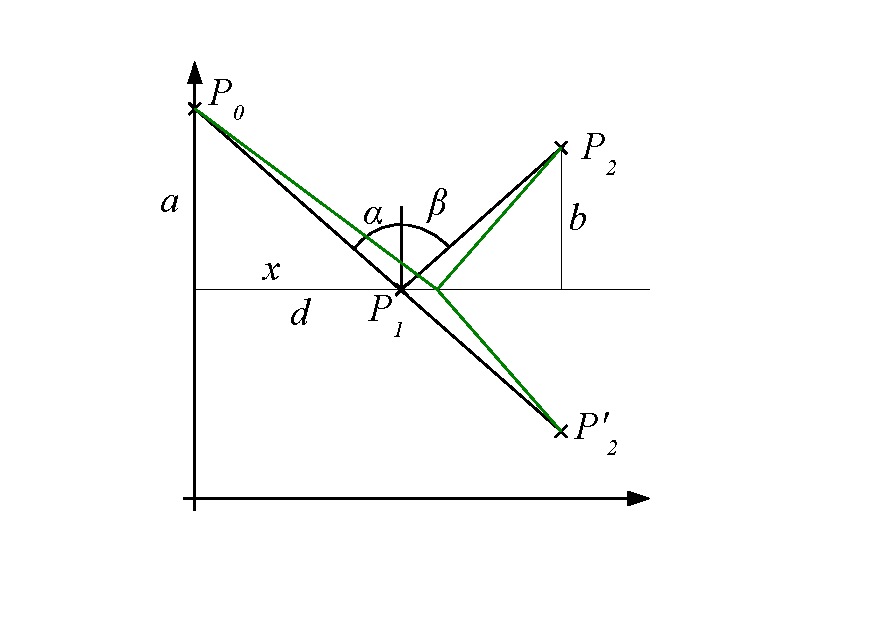
\includegraphics[width=0.7\textwidth]{licht/picture/Spiegelung.pdf}
	\caption{Skizze des Reflexionsgesetzes}
	\label{Ab:spiegelung}
\end{center}
\end{figure}
In \figref{Ab:spiegelung} ist ersichtlich, dass die Substitutionen
\ref{substitution1} und \ref{substitution2} von \secref{brechungsgesetz}
auch hier n"utzlich sind.
Nach etwas umformen ergibt sich, dass Eintritts- und Austrittswinkel
gleich sind (\eqref{brechung}).
\begin{equation}
0 = \sin(\alpha) - \sin(\beta) \quad \Leftrightarrow \quad \sin(\beta) = \sin(\alpha) \quad \Leftrightarrow\quad \beta = \alpha
\label{brechung}
\end{equation}
In \figref{Ab:spiegelung} ist ersichtlich, dass die Linie des Startpunktes
bis zum 
gespiegelten Endpunkt eine Gerade ist, welche der Funktion des k"urzesten
Weges entspricht.
